\documentclass[9pt,conference]{IEEEtran}

\usepackage[colorlinks,allcolors=blue]{hyperref}
\usepackage{listings}
\usepackage{graphicx}
\usepackage{amsfonts}
\usepackage{verbatim}
\graphicspath{{./images/}}

\begin{document}

    \title{Quality assurance of digital twins -- An experience report in the automotive industry}
    \author{
        \IEEEauthorblockN{
            Georg Hackenberg
        }
        \IEEEauthorblockA{
            School of Engineering\\
            University of Applied Sciences Upper Austria\\
            4600 Wels, Upper Austria, Austria\\
            \href{mailto:georg.hackenberg@fh-wels.at}{georg.hackenberg@fh-wels.at}
        }
        \and
        \IEEEauthorblockN{
            Alican Tüzün
        }
        \IEEEauthorblockA{
            School of Engineering\\
            University of Applied Sciences Upper Austria\\
            4600 Wels, Upper Austria, Austria\\
            \href{mailto:alican.tuezuen@fh-wels.at}{alican.tuezuen@fh-wels.at}
        }
    }
    \maketitle

    \begin{abstract}
        Digital twins are becoming more and more important for the efficient and effective development and operation of cyber-physical systems.
        However, digital twins are only useful if they reflect the real-world system accurately enough, i.e.\ their quality is high enough.
        This claim entails the question, of what the term quality in the context of digital twins means and how it can be measured.
        In this article, we present our experience with the quality assurance of a digital twin for an assembly line in the automotive industry.
        We explain our preliminary definition of digital twin quality, which we derive from classical quality models for general software systems.
        Furthermore, we describe quality issues, which we were able to detect in a digital twin of an assembly line in the automotive industry.
        Finally, we conclude how to leverage our experience in different contexts and how to generalize the underlying approaches.
    \end{abstract}

    \section{Introduction}\label{section:introduction}
    A popular but highly misunderstood notion with fuzzy boundaries is the `digital twin.' 
    The misunderstanding began with the Apollo 13 mission, which many authors claim, had a first digital twin The twin of Apollo 13 was merely a tangible replication of the spacecraft that has been utilized in the physical simulations. Even though the `digital' aspect was expected to be present, 
    it wasn't~\cite{GrievesApollo13}. The historic D-day map (also known as the Big Board) in Southwick House England, which was used simultaneously before and during operation, can be argued to be similar. 
    The board was a twin of the operation, and it included models of battalions and ships that reflected the actual locations of the corresponding formations. 
    Furthermore, synchronization was implemented with radio communication to give directives from the real system to control the operation flow and also to update the twin's state~\cite{AMRC}.

    To begin analyzing `the digital twin' and its quality, authors needed to come up with a concrete description that involved a great level of abstraction. 
    The definition of a digital twin given by the digital twin consortium, according to the authors, is the best one currently available: `A digital twin is a virtual representation of real-world entities and processes, synchronized at 
    a specified frequency and fidelity.'~\cite{digitaltwinconsortium2022}.

    What makes that definition the best? Because it provides the highest abstraction level among the definitions of digital twins that we discovered during our literature analysis. The following is a poor example of abstraction taken from the initial definition of a digital twin from NASA's roadmap from 2010: `A digital twin is an integrated multi-physics, multi-scale, probabilistic simulation of a 
    vehicle or system that uses the best available physical models, sensor updates, fleet history, etc., to mirror the life of its flying twin~\cite{NASA}.'
    The digital twins that we encounter nowadays don't typically fall under NASA's definition. We want to stress that NASA's definition of a  digital twin is accurate since digital twins are systems that are `context' centered. 
    This definition, therefore, is appropriate in the context of NASA's use case and is thus accurate, but the abstraction level is not sufficiently high to allow for a thorough understanding of digital twins.

    In addition, we would want to emphasize the significance of Grieves' 2006 description of digital twins in the PLM book,
    which traces the origins of the concept. Although it featured the same components as a digital twin at the time, it was known as an Information Mirroring Model (IM)~\cite{GrievesPLMBook}. 
    They decided to use NASA's Digital Twin rather than IM after co-authoring the article with Vickers.

    \begin{figure}
        \centering
        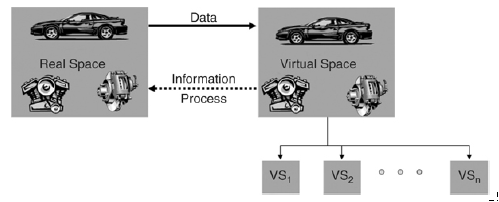
\includegraphics[width =0.45\textwidth]{GrievesInformationMirroringModel.png}
        \caption{Grieves Information Mirroring Model}
        \label{fig:GrievesInformationMirroringModel}
        \cite{GrievesPLMBook}
    \end{figure}

    \subsection*{Real System}

    The term `real system' in the context of digital twins refers to a system that is a tangible thing that has the characteristics of a system. Depending on the system's context, we can use black-box, gray-box, or white-box methodologies to study the system. 
    The usage of various artifacts by Grieves in a system he referred to as `real space' can be seen in Figure~\ref{fig:GrievesInformationMirroringModel}.

    \subsection*{Virtual System}
    Virtual refers to an existence that exists in a computer system as opposed to a physical system. Therefore, virtual systems are abstract systems, which are nothing but an abstraction of the real system.
    The term `abstract systems' refers to systems that have had their set of variables and functions `abstracted' so that they may be computed by a solver, which in this case solver could be either the human brain or a computer.
    Additionally, just because a system is an abstract system doesn't mean it lacks a physical body; rather, it is abstracted. 
    Virtual systems can't exist on their own since, like abstract systems, they require a medium to exist. Computer systems, a higher system of virtual systems, are an ideal medium for virtual systems.
    
    \subsection*{Connection Between the Real and Virtual System}
    If we step back and observe the consortium's definition in~\ref{section:introduction}, which we told is the best definition we could find, 
    it talks about synchronization, fidelity and some specified frequency. As can be guessed these terms are attributes of the real-virtual connection.
    Synchronization is used here instead of twinning, mirroring and connecting. 
    Real-time is a time value, which is most of the time a constant value and defines the update frequency of the state of the virtual system of interest relative to the system of interest.
    Fidelity is the degree of precision and accuracy of our digital twin, relative to the system of interest.
    These words are highly dependent on the context of the digital twin.
    \subsection{Research objective}
    Find an approach to assess the quality of Digital twins~\cite{Jones2020}

    \subsection{Research question}\label{section: Research Questions}
    What is the quality of digital twins?

    \subsection{Research methodology}
    TODO

    \section{State of the art on quality}
    TODO

    \subsection{Product quality}
    Most generic (e.g.~House of quality, ...)

    \subsection{Software quality}
    Medium (e.g.~ISO/IEC 9126 and ISO 25010, ...)

    \subsection{Digital twin quality}
    Most specific (a bit more research here!)

    \section{Initial approach in the FELICE project}
    Inspired by ISO 25010...

    \subsection{First criterion: Correctness}
    
    \subsubsection{Definition}
    Car vs airplane (with nice pictures!)

    \subsubsection{Motivation}
    TODO

    \subsubsection{Findings from FELICE}
    TODO

    \subsection{Second criterion: Completeness}
    
    \subsubsection{Definition}
    Car vs engine (with nice pictures!)

    \subsubsection{Motivation}
    TODO

    \subsubsection{Findings from FELICE}
    TODO

    \subsection{Third criterion: Fidelity}
    
    \subsubsection{Definition}
    Linear vs differential (with nice pictures!)

    \subsubsection{Motivation}
    TODO

    \subsubsection{Findings from FELICE}
    TODO

    \subsection{Fourth criterion: Efficiency}
    
    \subsubsection{Definition}
    1ms vs 1min (with nice pictures!)

    \subsubsection{Motivation}
    TODO

    \subsubsection{Findings from FELICE}
    TODO

    \subsection{Fifth criterion: Evolvability}
    
    \subsubsection{Definition}
    Effort to adapt the digital twin to new circumstances (e.g.\ add new machine, replace machine, etc.)

    \subsubsection{Motivation}
    TODO

    \subsubsection{Findings from FELICE}
    TODO

    \begin{comment}
        \section{Whatever}

        \subsection{Grieves Information Mirroring Model}

        \subsubsection{How it is defined?}

        His conceptual model is an ideal Product Lifecycle Management (PLM), has just one important goal which is to gather as much information about the actual space as feasible to minimize the waste of energy, time, and materials. 
        It is composed primarily of four parts. Real or physical space, virtual space, connections between real and virtual space, and virtual simulations.

        As we can see, it shares almost all of the same components as the digital twins of today. Virtual simulation is an optional component that Grieves subsequently removed to simplify the model. [GrievesEliminateForthElement] 
        The simple model version is indicated by the fact that only the first three (Physical System, Virtual System, and Connection Between Them) will be taken into account. 
        It should be mentioned that we shall define these three components in our own words using previous definitions of each component.  Additionally, by using the consortium's definition, we are simply improving the grieves IM model as a reference.
        The physical space is where we start first.

        \begin{figure}[htbp]
            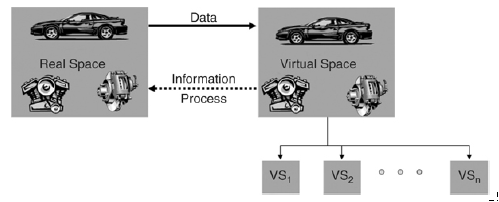
\includegraphics[width=\columnwidth]{Grieves Information Mirroring Model.png}
            \caption{Information Mirroring Model}
            \label{IM}
        \end{figure}

        \subsubsection{Why it is problematic?}

        TODO

        \subsection{Real System}
        We shall refer to a real system instead of calling it a real space. 
        Why? Because everything is an open system according to the system theory, 
        with the upper bound of the universe and lower bound as subatomic particles.
        As a result, the universe and subatomic particles can be viewed as closed systems, 
        simplifying definitions and facilitating the analysis of entities as systems. 
        In the literature, we see most of the time a notion called " entity" and sometimes an "artifact". 
        For instance, the digital twin framework developed by (TAO et al.) has both a physical and virtual entity.
        An entity is any separate and independent system, whether it be real or abstract.
        On the other hand, an artifact is a thing that humans have created or constructed. 
        Therefore, when we speak of entities, we really mean systems. 
        And when we discuss artifacts, we are still discussing physical systems but with the caveat of human interaction. 
        Automobiles, engines, software, artwork, food, and telephones are a few examples of artifacts.

        Above, we established the term "entity," but what about the physical connection of an entity? 
        Because an entity could be a physical system or an abstract system. 
        We won't go into further depth about these two distinct ideas, but just so you know, 
        when we talk about physical systems, we do not include abstract systems that require a
        media to exist, such as ideas, texts, diagrams, and mathematics, which are nothing more than abstractions.

        The term "real system" in the context of digital twins refers to a system that is a tangible thing and also has 
        the characteristics of a system. The usage of various artifacts by Grieves in a system he referred to as `real space' 
        can be seen in figure X. 
        For convenience, we'll refer to this system as a "real system" or, as Mobus prefers to say, a `system of interest.'. 
        Instead of using black-and-white images, we instead created subsystems out of circles, each of which represented an artifact. 
        It is clear to see that every subsystem (artifact) includes smaller subsystems as well. 
        Once more using Grieves' example, an automobile(an element of the real space according to figure 1), 
        which is an artifact, that includes several parts, including a radio, a motor, wheels, etc. 
        Additionally, these subsystems (artifacts) can be further broken down into even smaller subsystems, 
        down to subatomic particles, which, as we mentioned above, is the lowest we can go in terms of the system theory. 
        But the question is, should we break things down to the level of subatomic particles to comprehend the system? Considering digital twins, 
        the answer is a resounding no.

        Consequently, why bother to define these terms? Because the granularity of the digital twin is determined by the complexity of the real system. 
        In the end, a System of Interest is what we'll be twinning! Of course, the system of interest is not as simple to define as in figure X. 
        One crucial component and stage of the digital twin is to comprehend how the real system, or more precisely the system of interest, 
        actually functions. How can one know what to twin if it is not well understood?
        The system of interest can be analyzed in three different ways. If we don't have the opportunity to examine the inner workings of the system, 
        we can use the black boxing technique, which focuses primarily on the mathematical (and frequently statistical) 
        relationships between inputs and outputs. This method doesn't provide insight into the inner workings of the system, but it still provides 
        a basic grasp of how a system operates. If the system exhibits linear behavior, it works great.

        The second method, known as the gray box method, examines the inner workings of comparable systems that should be `like' 
        the system of interest to understand how the inner workings of a similar system react when various inputs are applied and the results of the system are monitored. 
        This method is used for the majority of biological work, such as the experiments medical students conduct on cadavers to learn how the human body functions. 
        
        The final method, known as the `white box method,' is better than the others since it examines every system's component. 
        The interesting thing to realize is that the system's integrity(Objectiveness) shouldn't be impaired.
        What objectiveness means is that while the system functions as a whole, we should also study the relationships 
        between the subsystems in addition to the subsystems themselves. 
        Observing our galaxy is a fantastic example. Telescopes allow us to individually assess the condition of the subsystems (planets, solar systems) 
        without affecting the overall system.

        Physical space, as a whole, is a physical system (which we refer to as the system of interest),
        with subsystems and linkages between them. Depending on the SOI's context, we can use black box, gray box, or white box methodologies to study the system.
        In addition, I wish to draw attention to the fact that the SOI's details are not fully depicted in figure 2. 
        For additional details on the system theory, we strongly advise reading `von Bertalanffy 2003'.

        \begin{figure}[htbp]
            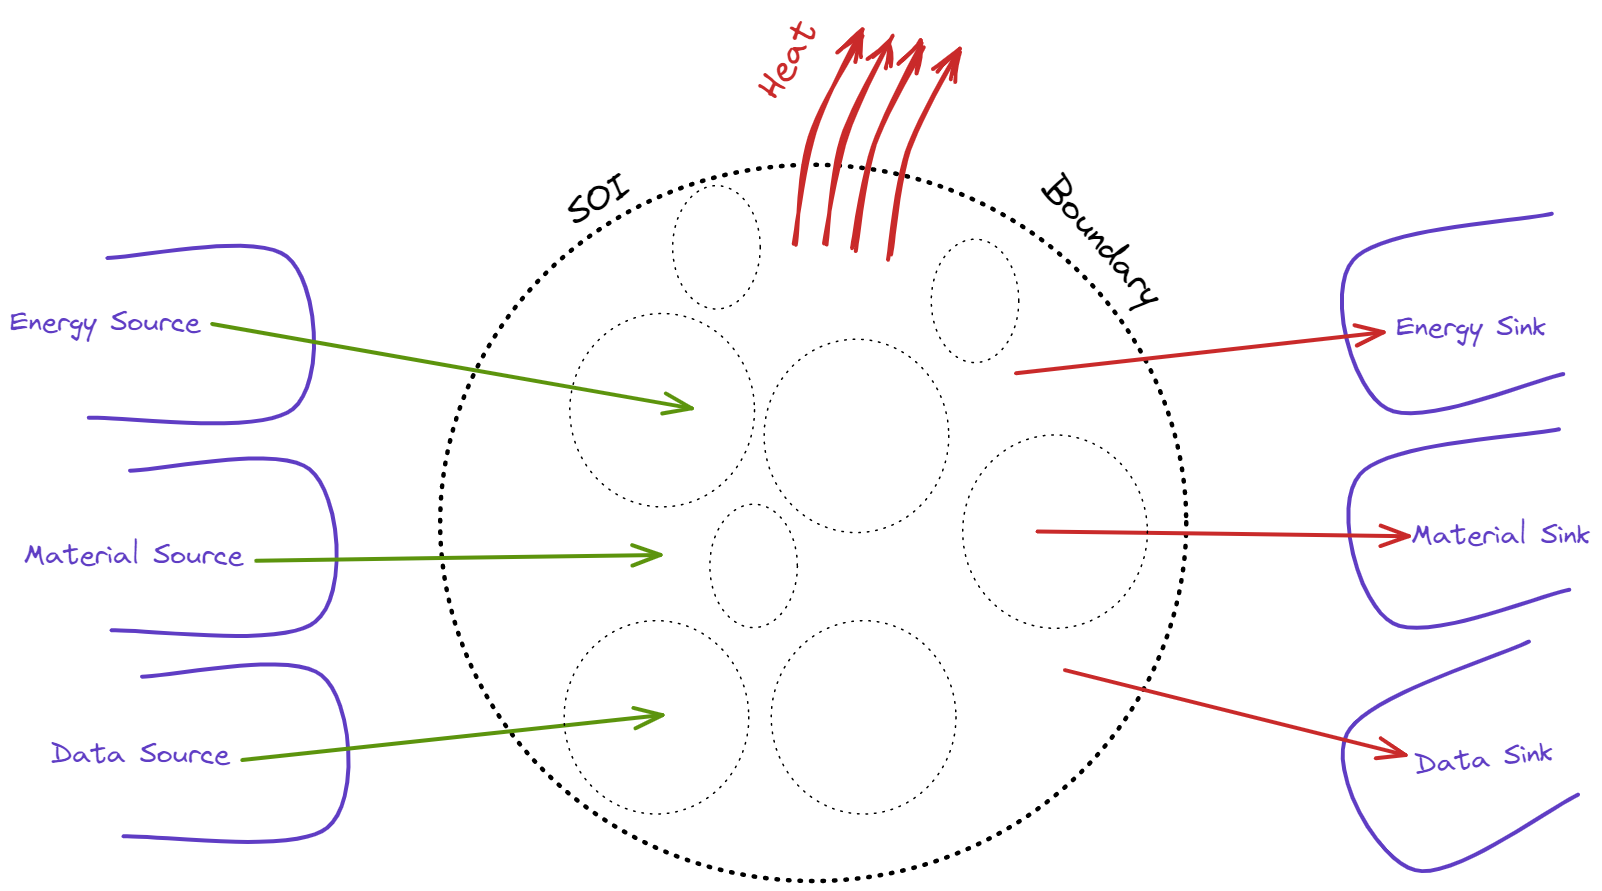
\includegraphics[width=\columnwidth]{SOI.png}
            \caption{System Of Interest}
            \label{SOI}
        \end{figure}

        \subsection{Virtual System(Digital Twin)}

        First of all, what does the term `virtual' mean? Virtual refers to an existence (or entity?) that exists in a computer system as opposed to a physical system. 
        Therefore, we made sure to note that we are not speaking of abstract systems when we described physical systems. 
        We also discussed the distinction between an entity and an artifact. The term `abstract systems'  refers to systems that have had their set of variables and functions 
        `abstracted'  so that they may be computed by a solver, which in this case could be either the human brain or a computer.
        Additionally, just because a system is abstract doesn't mean it lacks a physical body; rather, as we previously established, 
        it is abstracted. Computers, symbolic language, and the human mind all can contain these abstract systems.
        Symbolic text in this sense covers not only text on the sheet but also mathematical symbols, logic, etc.

        Virtual systems can't exist on their own since, like abstract systems, they require a medium to exist.
        Computer systems, a higher system of virtual systems, are an ideal medium for virtual systems. 

        \begin{figure}[htbp]
            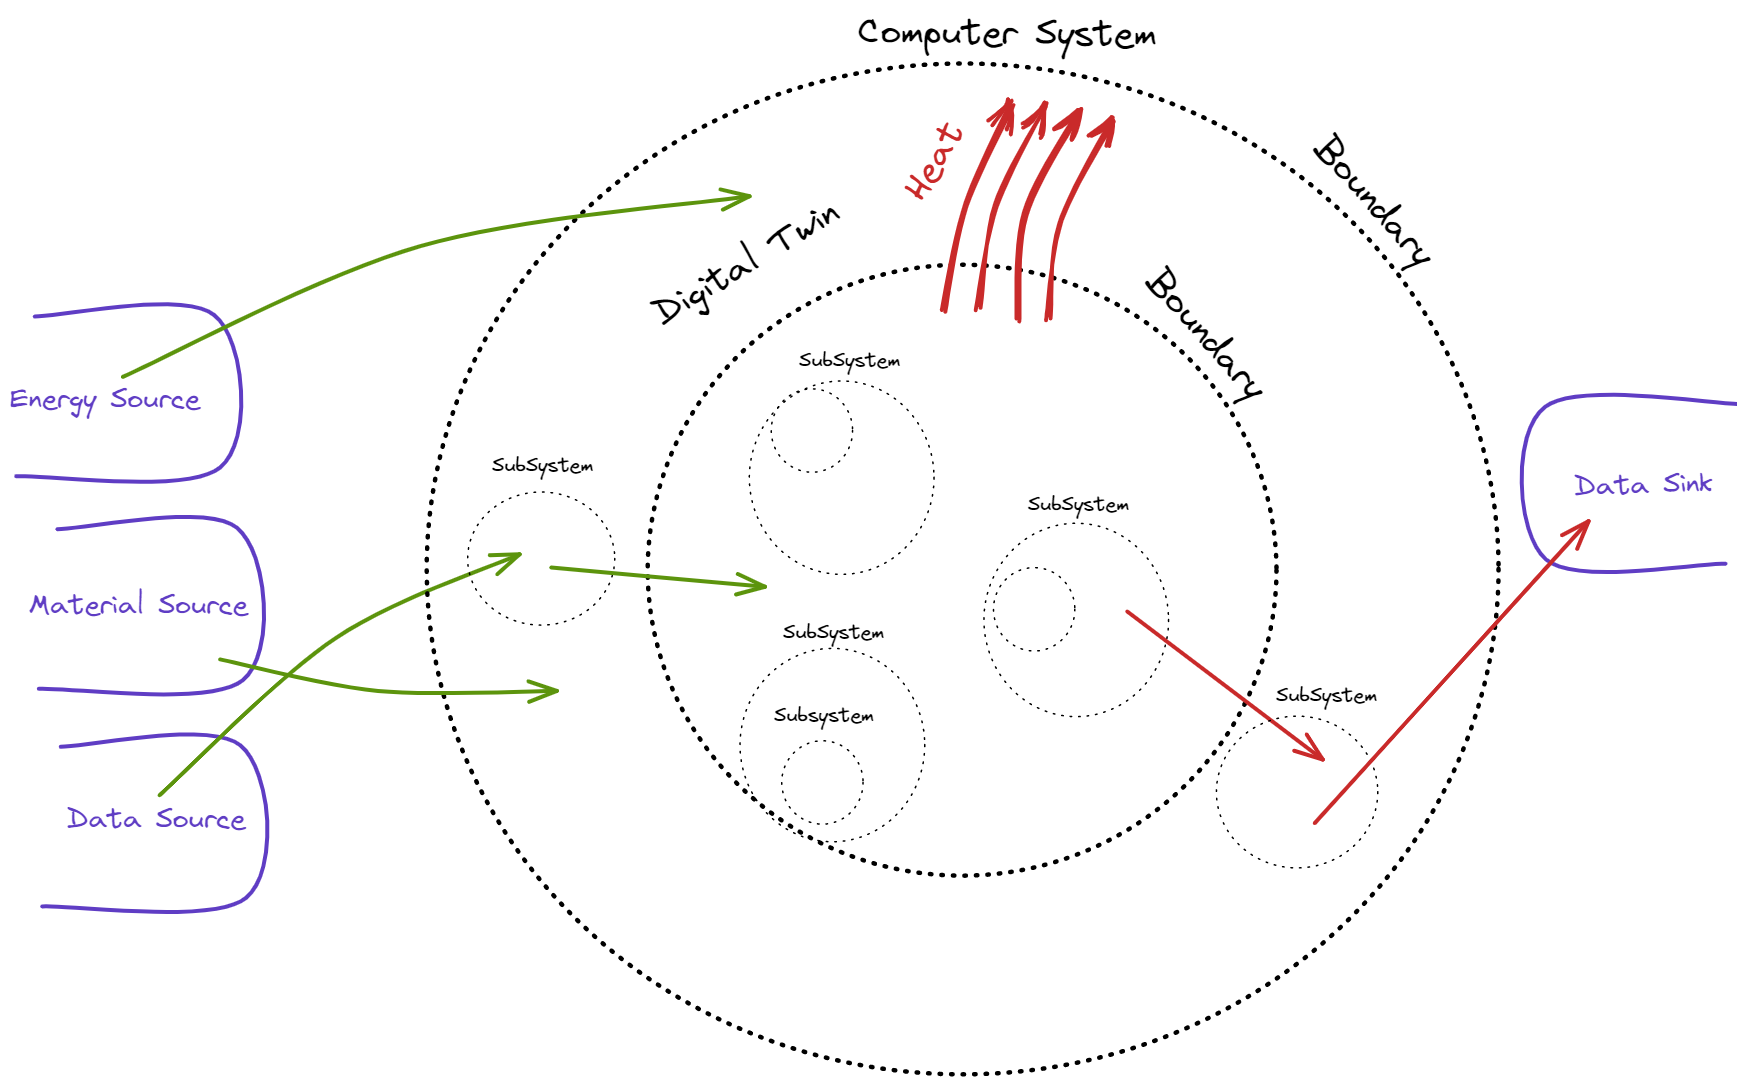
\includegraphics[width=\columnwidth]{DT SOI.png}
            \caption{Digital Twin SOI}
            \label{DTSOI}
        \end{figure}

        Recall that Grieves referred to the virtual system as a virtual space in figure 1. 
        We refer to it as a virtual system because it can only exist inside a computer system. 
        Additionally, we refer to the entities he depicted in the virtual space as virtual subsystems rather than the virtual entities he used. In figure 3, 
        we were creative and wrote `digital twin'  rather than `virtual system.'  Where does this digital twin emerge from?

        We must first understand what digital implies to comprehend the concept of a digital twin.  
        The term `digital has been in use since the late 14th century and is derived from the Latin word `digitus, ' 
        which means `finger'  or `toe.'. It gained popularity after digitalization in the 20th century and refers to the use of discrete digits to represent data. 
        Digital images, for instance, are represented by a matrix of pixels, which are nothing more than 8-bit integer values between 0 and 255 which represent the intensity 
        of the pixel. 
        We will therefore have digital models if we can digitally model our models. 
        Therefore, we will have digital models if we can digitally model our models. Where are these digital models being created? Throughout the digital system! 
        This system is referred to as a `digital twin'  since it is a digital twin of the SOI that is represented in the computer system.

        The reader will quickly and easily comprehend that a computer system may have several digital twins, 
        and that these systems may also be connected in some way, 
        creating yet another system that is also referred to as a digital twin. 
        Another immediate realization is that perhaps we won't have our SOI yet, 
        so how can we twin something that doesn't exist? Although the term we preferred was the best definition (for us), 
        it does not directly address the second question. In reality, most of the time, 
        the physical product will not be ready or not present to make a digital twin out of it. 
        But if we could have some data about the physical system, for example how it should look, 
        how much weight it should have, approximate dimensions and so on,  we can start constructing our system abstractly, 
        within the computer systems, with diagrams, or with using symbolic language. 
        But the important point is that everyone, who works on this abstract system should have a singular reference so that it can be constructed. Also after the construction, 
        still a real system is needed to validate and verify. Most frequently, this viewpoint is referred to as a prototype digital twin. And if the SOI is present its called instance digital twin.
        
        So far, we inspected the real system (system of interest), and virtual system. 
        As we talked about above, there is a third part which is a connection between the real system and the virtual system, which we will explain next.
        
        \subsection{Connection Between the Systems}

        \subsection{Possibility of States}
        \subsection{Context of Digital Twin}
        \subsection{Quality of Digital Twin}
    \end{comment}
    
    \begin{comment}
        \section{Literature review}
        \label{section: literature}
        Literature analysis was executed, to analyze current DT literature within the concept of digital twin quality. The analysis especially focused on 
        how the digital twin quality is mentioned and assessed within the academic dissertations.

        Methodology (see Section~\ref{section:liteature_methodology}), Result (see Section~\ref{section:liteature_result}), and Summary (See Section~\ref{section:liteature_summary})...

        \subsection{Methodology}
        \label{section:liteature_methodology}
        Google Scholar (GS), Scopus (SCP) and Research Rabbit (RR) tools are used to fulfill our requirements for the literature review. 
        Since there is a great number of digital twin publications in academics, 
        narrowing the research is necessary, so the following algorithm which can be seen in Figure \ref{fig:literaturesearchalgorithm} with several levels of filtering will be applied.
        
        First filtering will be done with the following criteria:
        \begin{itemize}
            \item Dissertations should be written in English and published in a journal/conference.
            \item Dissertations should not be older than 2018
            \item Search term should be exactly searched.
        \end{itemize}

        Filtering query calls for the GS and SCP are the following:
        \begin{itemize}
            \item Google Scholar = "search term"
            \item Scopus = ALL ( "digital twin quality" ) AND PUBYEAR > 2018 AND PUBYEAR < 2023 AND ( LIMIT-TO (LANGUAGE , "English" )) 
        \end{itemize} 

        Also want to note that, in the GS, there isn't a function that filters the dates, instead the user should click the Since 2018 option to filter the dates.

        Second filtering will be done to eliminate the duplications and even though authors already filtered the search for the English language,
        still some results without the English language will appear. Again, language filtering should be done to clean the results.
        \begin{itemize}
            \item Remove Duplications
            \item Remove the dissertations which are not English manually
        \end{itemize}  
        
        After the second filtration, the third filtering which is a manual investigation should occur with the following filtering criteria:
        \begin{itemize}
            \item Proper literature review should be present in the selected dissertation
            \item Abstract and conclusion should be relevant to the search term
        \end{itemize}
        
        If an interesting dissertation(s) would be found during the reading, it will be checked again with the first filter.
        \begin{figure}
            \centering
            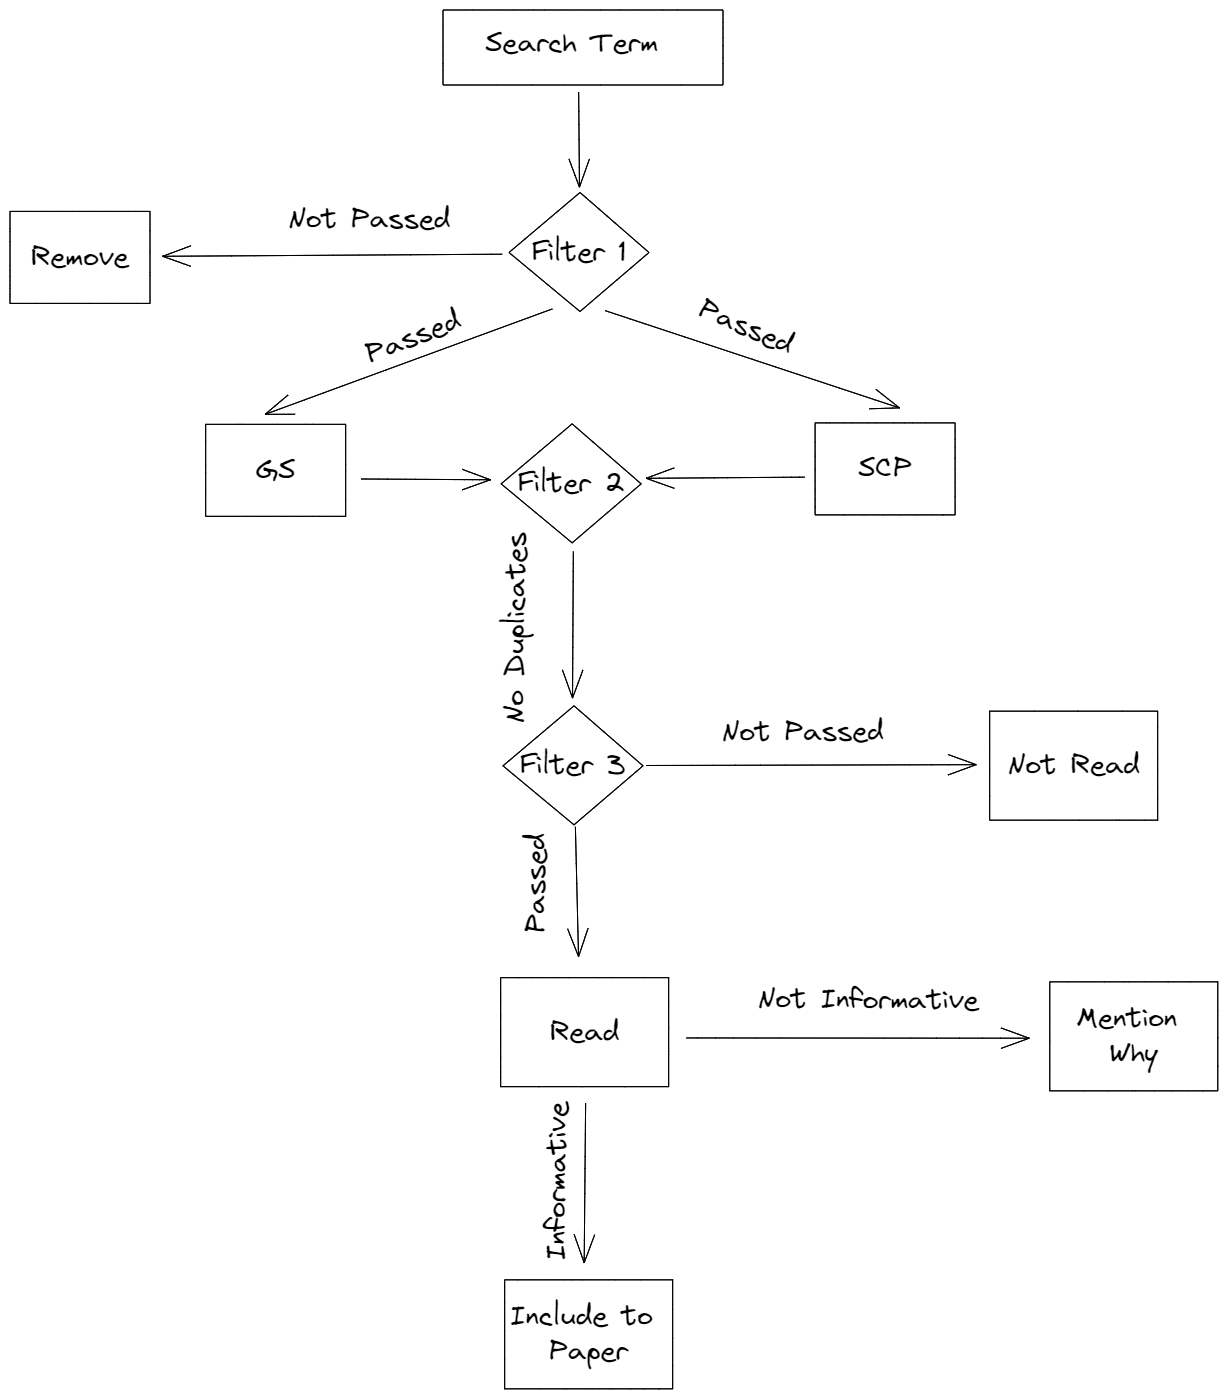
\includegraphics[width =0.45\textwidth]{LRMethod.png}
            \caption{Literature Search Algorithm}
            \label{fig:literaturesearchalgorithm}
        \end{figure} 
        \begin{figure}
            \centering
            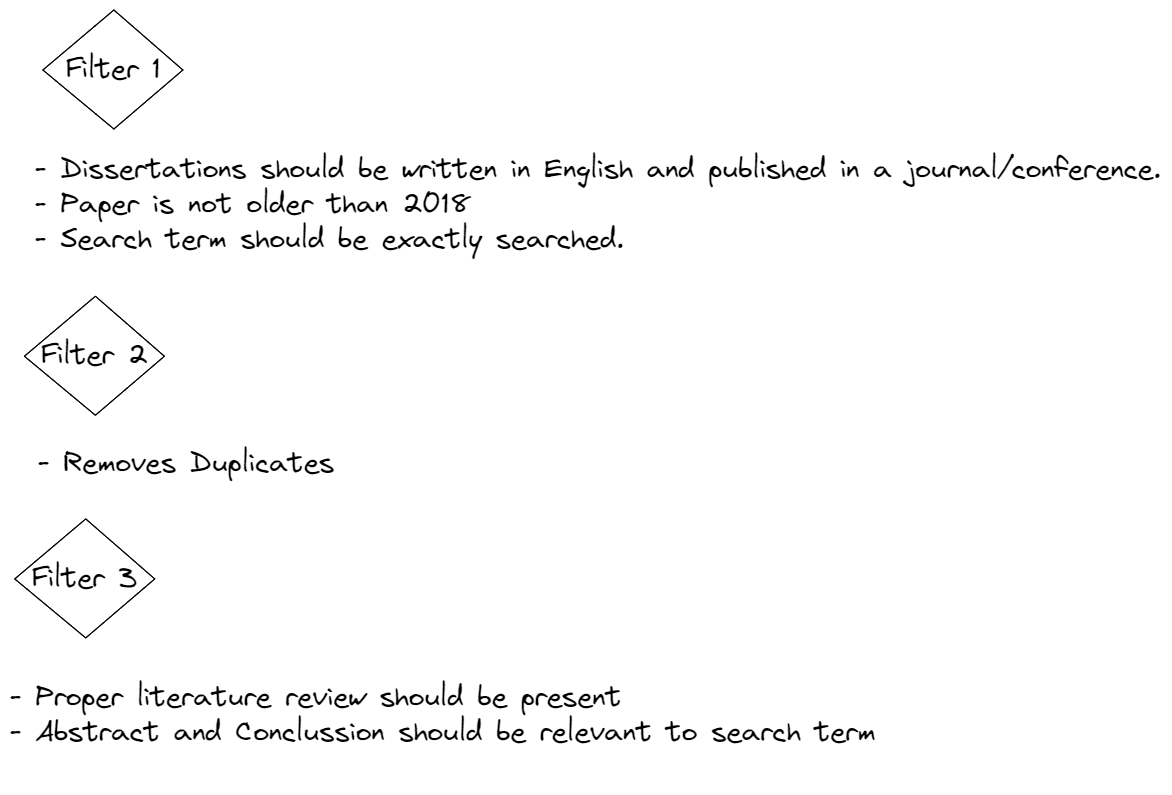
\includegraphics[width =0.45\textwidth]{LRMethodLegacy.png}
            \caption{Literature Search Algorithm Legend}
            \label{fig:literaturesearchalgorithmlegend}
        \end{figure}
        
        \subsection{Result}
        \label{section:liteature_result}
        The following results were achieved by selecting several search terms.
        
        \subsubsection*{Digital Twin Quality}
        \label{subsection:DigitalTwinQuality}
        First filtering was done for the search term "digital twin quality", meanwhile GS gave 41 different results, and SCP gave only 3 results.
        After the second filtering process, 3 duplications and 31 different results were found. 10 dissertations were not in English.
        After the third filtering process, 9 dissertations passed and the rest is rejected.

        \subsubsection*{Digital Twin Model Verification}
        \label{subsection:DigitalTwinVerification}

        \subsubsection*{Digital Twin Model Validation}
        \label{subsection:DigitalTwinValidation}
        %What is the existing literature?

        \subsection{Summary}~\label{section:liteature_summary}
        What do we learn from existing literature?

        He Zhang et al.introduced a consistency evaluation method for digital twin models, which can be used to assess the quality of the digital twin ~\cite{Jones2020}.
        (Existing literature does at most partially solve our problem!)
    \end{comment}

    \section{Future approach in the FELICE project}
    \label{section:framework_1}
    TODO

    \begin{figure}[htbp]
        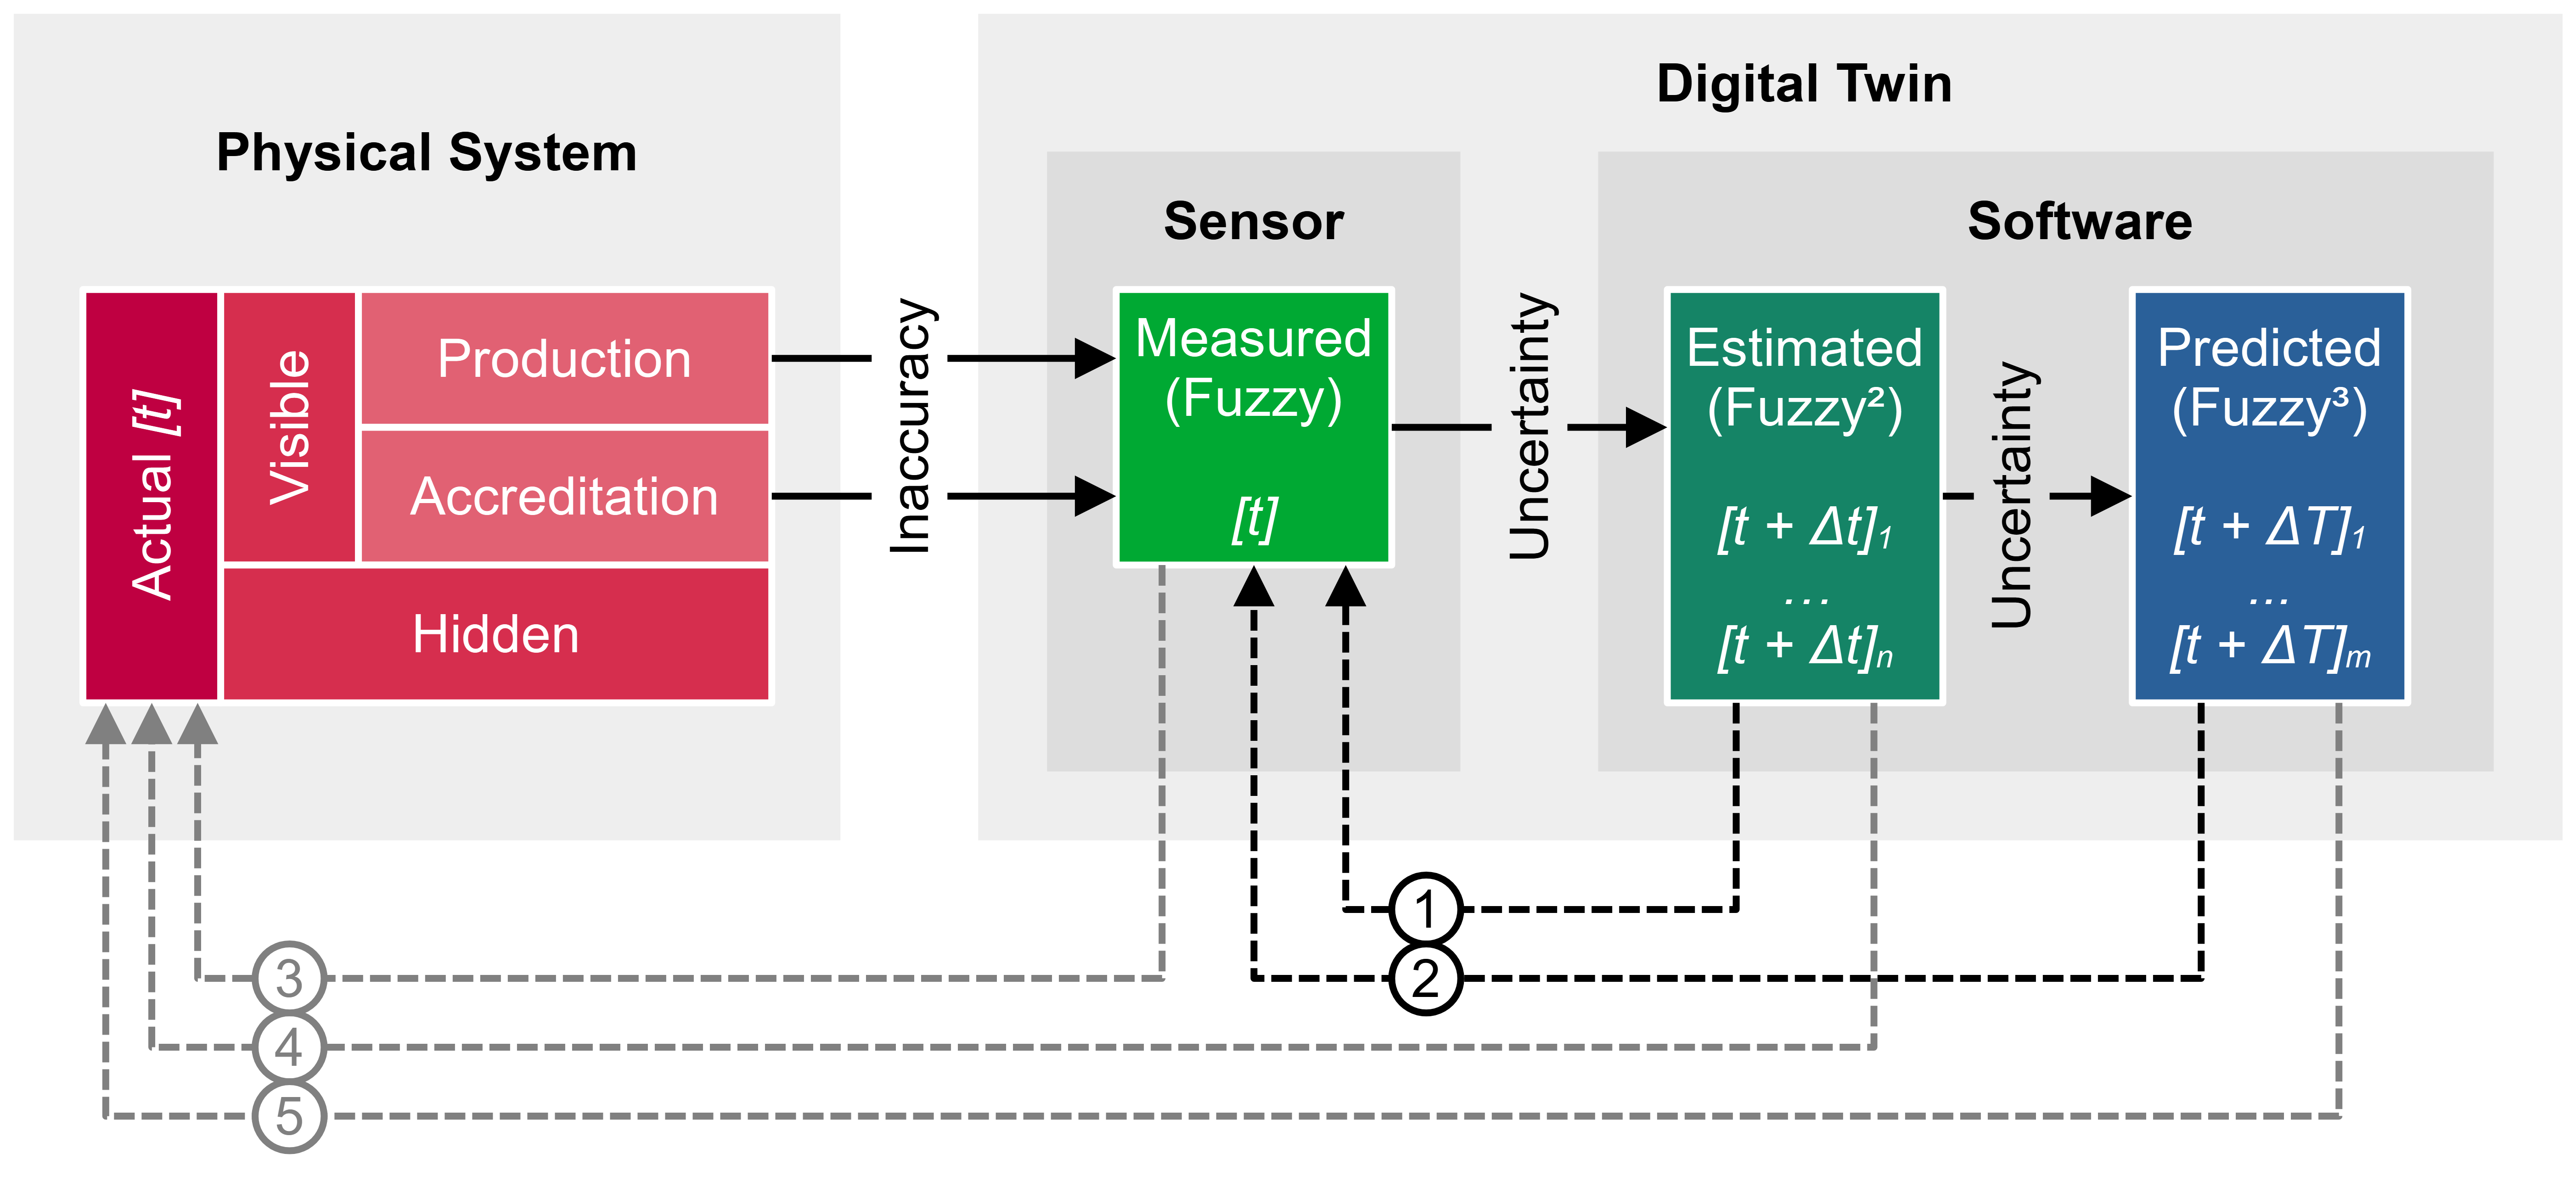
\includegraphics[width=\columnwidth]{Digital Twin Deviation.png}
        \caption{TODO}
        \label{todo-2}
    \end{figure}

    \begin{figure}[htbp]
        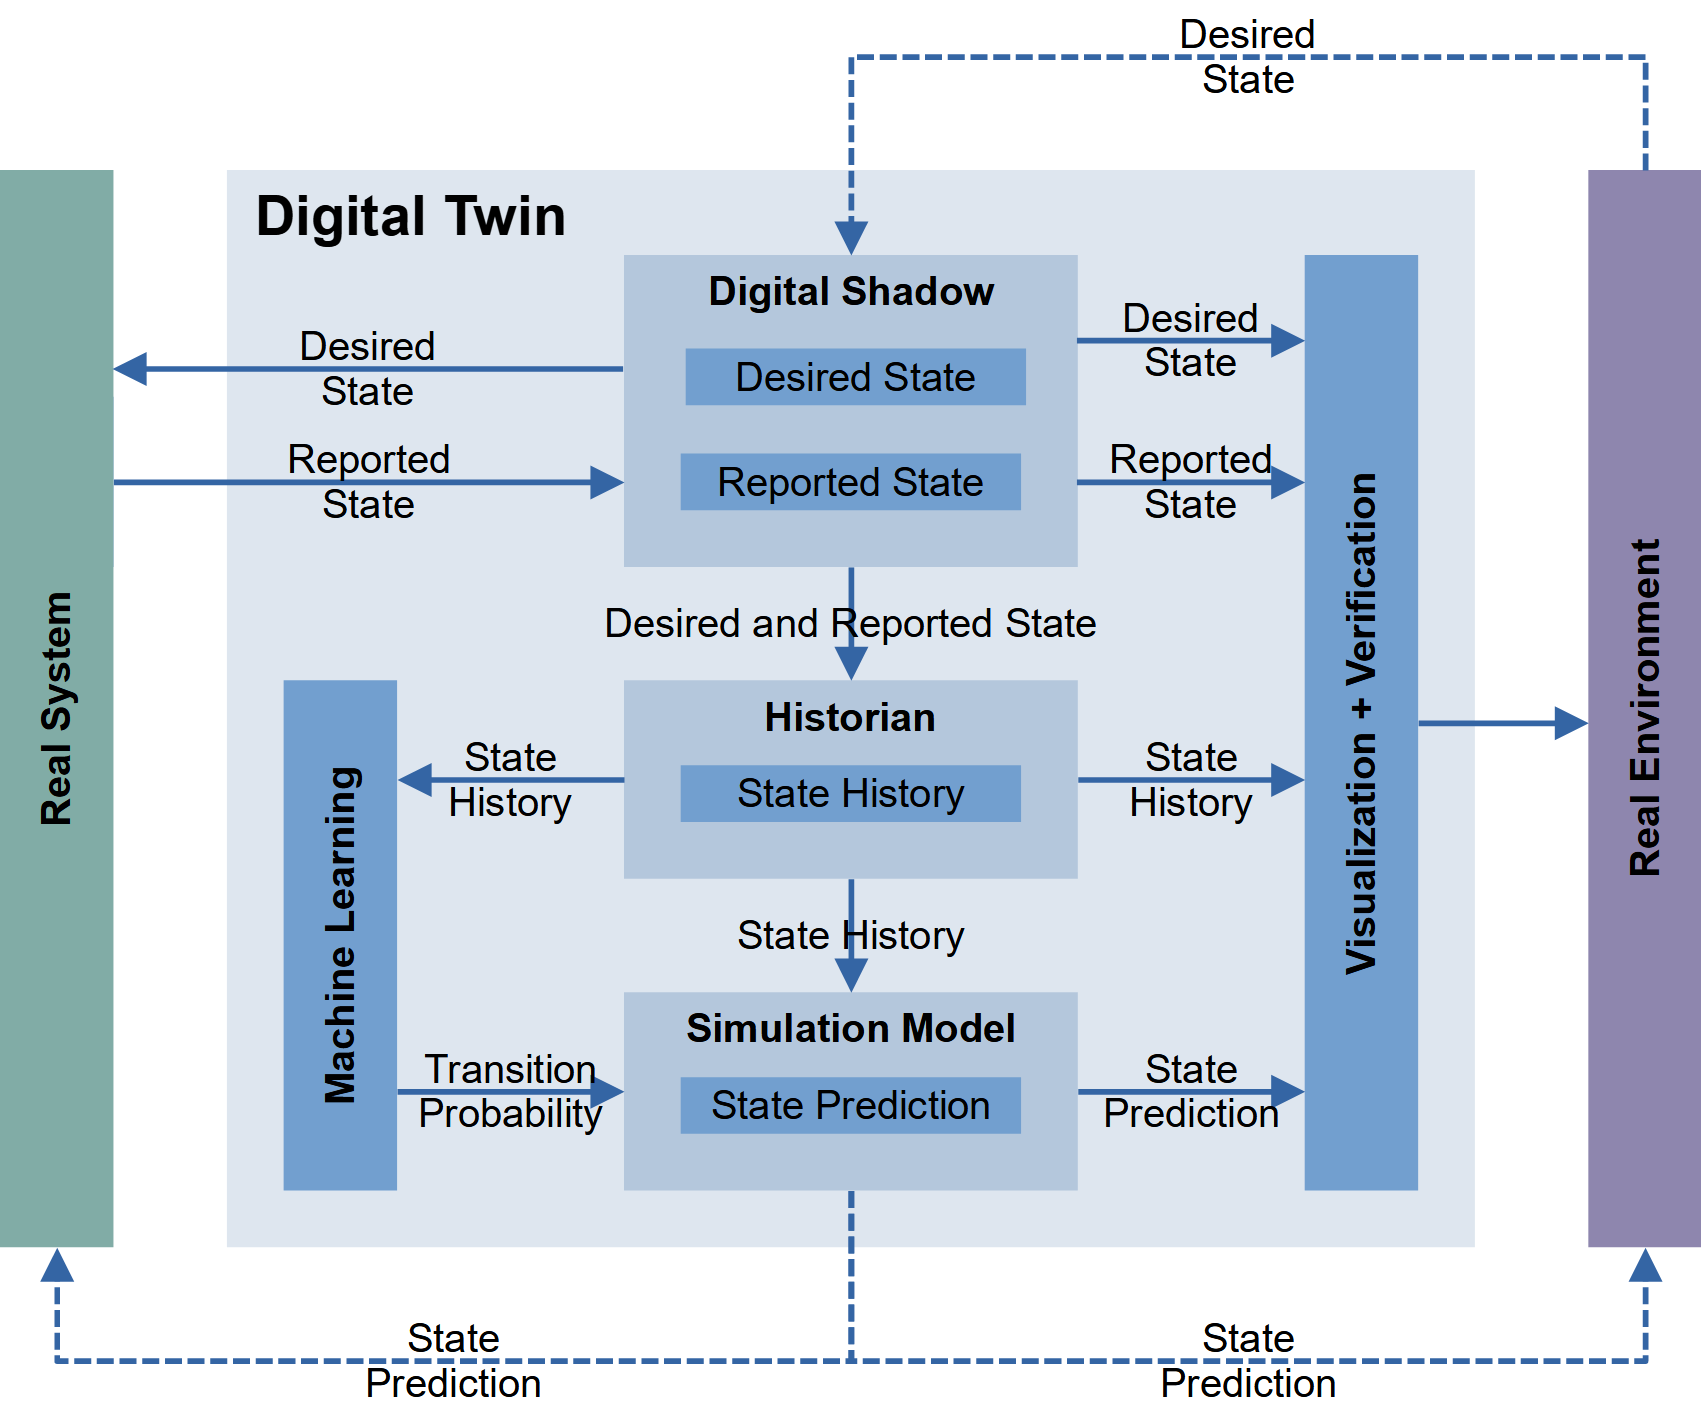
\includegraphics[width=\columnwidth]{Digital Twin.png}
        \caption{TODO}
        \label{todo-1}
    \end{figure}

    \begin{figure}[htbp]
        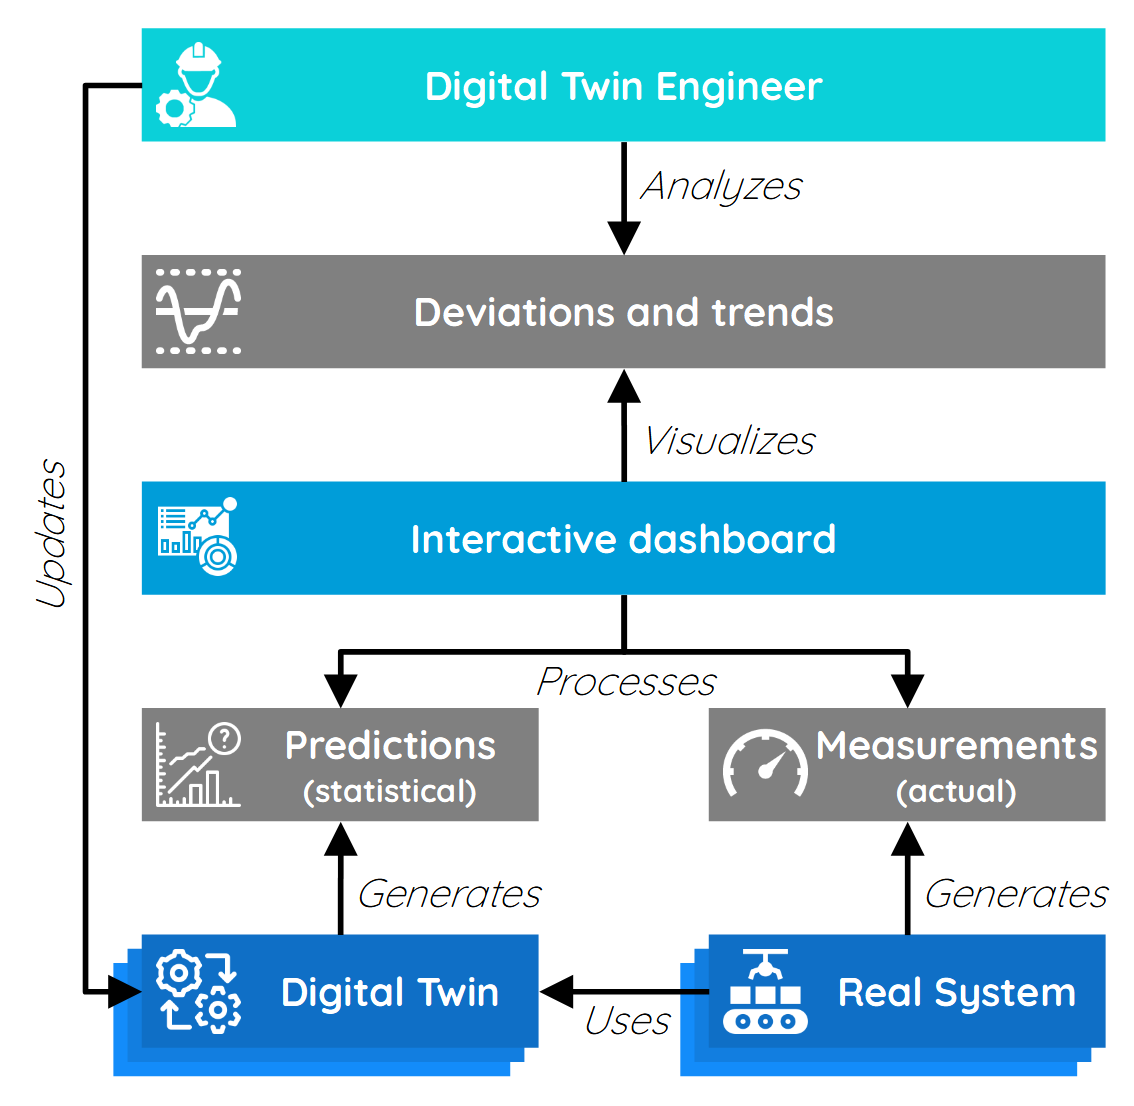
\includegraphics[width=\columnwidth]{Continuous Quality Control.png}
        \caption{TODO}
        \label{todo-3}
    \end{figure}

    \begin{comment}
        \section{Case study (FELICE)}\label{section:case}
        TODO (Explain the limitations of the FELICE digital twin! It is not a complete digital twin according to literature! It includes this, it is missing this.)

        \subsection{Methodology}~\label{section:case_methodology}
        TODO

        \subsection{Result}~\label{section:case_result}
        TODO

        \subsection{Summary}~\label{section:case_summary}
        TODO
    \end{comment}

    \section{Conclusion}~\label{section:conclusion}
    TODO

    \section*{Acknowledgements}
    TODO

    \bibliography{main}
    \bibliographystyle{plain}

\end{document}